% threepennygui-Ht.tex
\begin{hcarentry}{threepenny-gui}
\label{threepenny-gui}
\report{Heinrich Apfelmus}%11/16
\status{active development}
\makeheader

Threepenny-gui is a framework for writing graphical user interfaces (GUI)
that uses the web browser as a display. Features include:

\begin{compactitem}
\item \emph{Easy installation.} Everyone has a reasonably modern web browser
  installed. Just install the library from Hackage and you are ready to go.
  The library is cross-platform.
\item \emph{HTML} + \emph{JavaScript}. You have all capabilities of HTML at
  your disposal when creating user interfaces. This is a blessing, but it can
  also be a curse, so the library includes a few layout combinators to quickly
  create user interfaces without the need to deal with the mess that is CSS. A
  foreign function interface (FFI) allows you to execute JavaScript code in
  the browser.
\item \emph{Functional Reactive Programming (FRP)} promises to eliminate the
  spaghetti code that you usually get when using the traditional imperative
  style for programming user interactions. Threepenny has an FRP library
  built-in, but its use is completely optional. Employ FRP when it is
  convenient and fall back to the traditional style when you hit an impasse.
\end{compactitem}

\subsubsection*{Current status}

The project is alive and kicking, the latest release is version
\verb`0.7.0.0`. You can download the library from Hackage and use it right
away to write that cheap GUI you need for your project. Here a screenshot from
the example code:

%**<img width=700 src="./chat.jpg">
%*ignore
\begin{center}
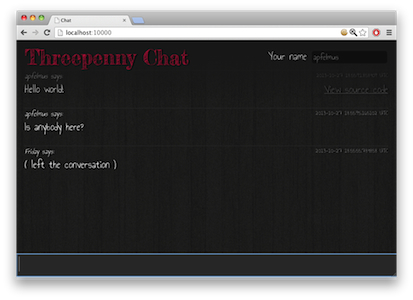
\includegraphics[width=0.5\textwidth]{html/chat.jpg}
\end{center}
%*endignore

For a collection of real world applications that use the library, have a look
at the gallery on the homepage.

Compared to the previous report, performance has been improved by reducing the communication from the browser to the server when creating new HTML DOM elements. Other than that, only minor changes have been made.
In particular, the library has been updated to work with the current Haskell ecosystem.

\subsubsection*{Future development}

The library is still very much in flux, significant API changes are likely in future versions. Future goals include:

\begin{itemize}
    \item Improve performance by batching FFI calls.
        This has already been partially implemented,
        but more library calls should be made batchable.
    \item Integrate with \href{http://electron.atom.io/}{Electron}, a new framework for developing desktop applications with HTML and JavaScript.
\end{itemize}

\FurtherReading
\begin{compactitem}
\item Project homepage: \url{http://wiki.haskell.org/Threepenny-gui}
\item Example code: \url{https://github.com/HeinrichApfelmus/threepenny-gui/tree/master/samples#readme}
\item Application gallery: \url{http://wiki.haskell.org/Threepenny-gui#Gallery}
\end{compactitem}
\end{hcarentry}
